%!TEX root = ../../thesis.tex
\section{Synthesizers}
\label{sec:webaudio-synth}
\begin{quote}
  ``I knew that it could be a sound of the future but I didn't realise how much the impact would be.'' - Giorgio Moroder
\end{quote}

The term `synthesizer' describes music instruments that create sounds solely electronically. The term was coined in the late 1960s by Robert A. Moog, founder of Moog Music the pioneering company in the field of analog synthesizers \cite[p. 67]{pinch2004analog}. Moog decided to call it `synthesizer', although the term was used before for another instrument, the `RCA synthesizer' which was also used to synthesize sounds, but which did not have the ability to be played in real-time, it needed to be programmed\footnote{\cite[p. 67]{pinch2004analog}}. Moog's synthesizers were modular synthesizers, meaning they consisted of individual modules that had to be patched together with wires in order to route the audio signal through filters and envelopes before it was sent to the speakers. The sound was created from electronic oscillators which were triggered by a keyboard that was attached to the synthesizer\footnote{\cite[p. 25ff]{pinch2004analog}}. Synthesizers were made famous in popular music in the 1970s by acts like Kraftwerk and Giorgio Moroder, who wrote the possibly most famous synthesizer-based song of that time: `I Feel Love' performed by Donna Summer \cite[14:37min]{bbc2009synthbritannia}. Since the first introduction of synthesizers in the 1960s, their architectures changed a lot and in addition to analog synthesizers, digital synthesizers and software synthesizers have been introduced. Today, synthesizers build the foundation of modern electronic music and they can be found in all DAWs.

There are many different ways how synthesizers can be implemented and they base on different theoretical approaches. This chapter will however focus on the background theory of analog synthesizers and only mention other approaches briefly.

Analog synthesizers, such as the ones that were created by Moog (Minimoog, Moog Modular etc.), are based on the concept of `subtractive synthesis'. In `subtractive synthesis', rich audio signals are taken and then manipulated to make them sound `less rich'. `Less rich' in this context does however not mean that the sound signal becomes less appealing to listeners. It means that the spectrum of the signal is reduced and that certain parts are emphasized, while other parts are left out \cite[p. 223f]{park2009introductionto}. The concept of the `subtractive synthesis' stands in contrast to the `additive synthesis', in which simple signals are added up to produce a more rich sound\footnote{\cite[p. 277f]{park2009introductionto}}.

\medskip

\begin{figure}[htb]
  \centerline{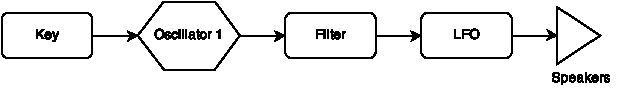
\includegraphics[width=\linewidth]{images/SimpleSynth.pdf}}
  \caption[A simple synthesizer's node graph]{A simple synthesizer's node graph}
  \label{fig:simple-synth-node-graph}
\end{figure}

The simplified node graph in \reffigure{fig:simple-synth-node-graph} shows how the signal's `richness' is shaped by the  different components of a synthesizer. The source of the signal is a raw oscillator (see \refchapter{sec:webaudio-osc}) signal which is initialized by pressing a key on the keyboard. Typically, a module that translates keys, which of course stand for musical notes, to the corresponding frequency lies in between the key and the oscillator. The oscillator's signal is then altered by a filter (see \refchapter{sec:webaudio-filter}) in order to remove some frequencies and in order to emphasize certain other frequencies. Next, the signal is routed into a Low Frequency Oscillator (LFO). The LFO's signal is used to modulate the amplitude or the pitch of the incoming signal in order to produce an alternating sound signal. The impact of this effect is determined by the LFO's frequency, which typically lies at the lower end of the human hearing. Humans would not be able to hear signal with this frequency, but the modulation of the input signal makes the alternations audible. The resulting signal is then routed to the speakers or to an audio-out port.

All parts from the above explained node graph can be implemented by using the Web Audio API's building blocks and build on top of them. \refchapter{impl-synth} will show which parts of the API could be reused and which could be combined to implement a synthesizer for the audio editor.